\subsection{The data}
	There are two groups of datasets.
	
	\subsubsection{Atmospheric aberration related}
	
		There are 4 datasets composed by PSFs and their corresponding PL intensities.
		
		\subparagraph{PSFs}
			The PSFs' electric fields are stored in a 3d matrix of depth 2: depth 1 and 2 represent the real and imaginary value of the electric field in a point.
			\begin{itemize}
				\item \textbf{Original sized PSFs}: A dataset of 70000 electric fields stored in 128x128x2 matrixes.
				\begin{figure*}[ht!]
					\centering
					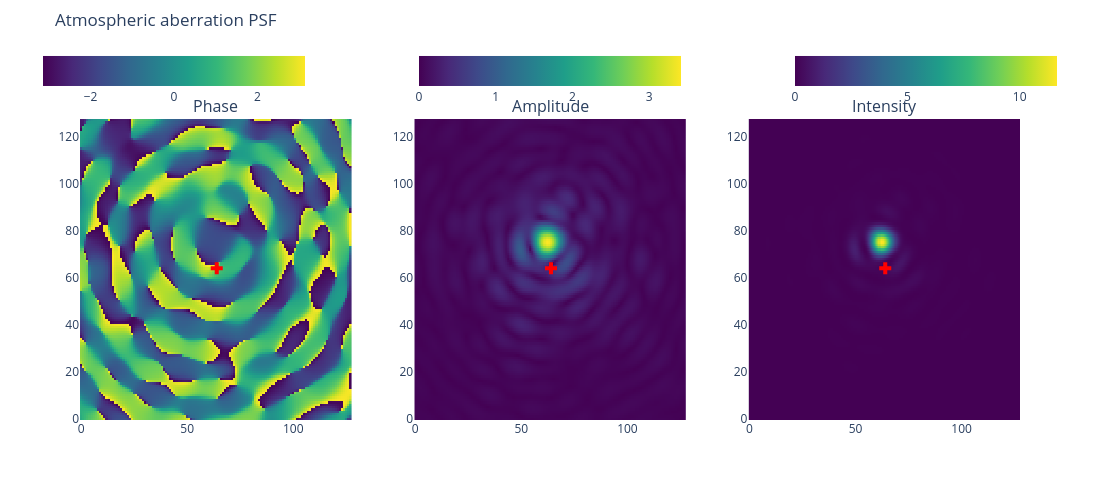
\includegraphics[width=0.4\textwidth]{pid-atmosphericaberrationpsf.png}
					\caption{Example original sized PSF}\hspace{\fill}
				\end{figure*}				
				\item \textbf{Cropped sized PSFs}:  A dataset of 70000 electric fields stored in 64x64x2 matrixes. These cropped  PSFs correspond to the central pixels from the Original sized PSFs.
				\begin{figure*}[ht!]
					\centering
					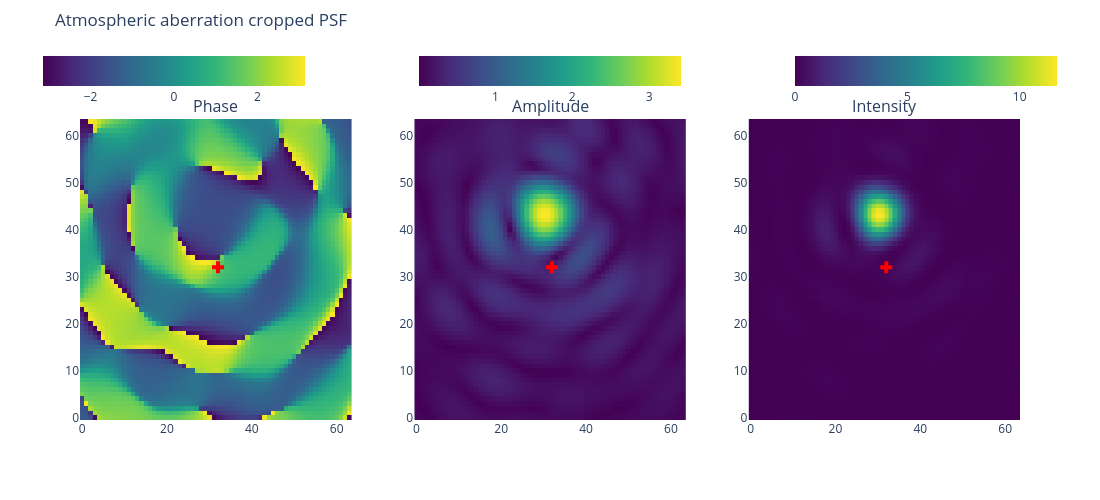
\includegraphics[width=0.4\textwidth]{pid-atmosphericaberrationcroppedpsf.png}
					\caption{Example Cropped sized PSF}\hspace{\fill}
				\end{figure*}			
				\item \textbf{Original sized predicted PSFs}:  A dataset of 70000 predicted electric fields stored in 128x128x2 matrices. These predicted PSFs are the outputs of a model trained with the Original PSFs dataset and their corresponding PL intensities.
				\begin{figure*}[ht!]
					\centering
					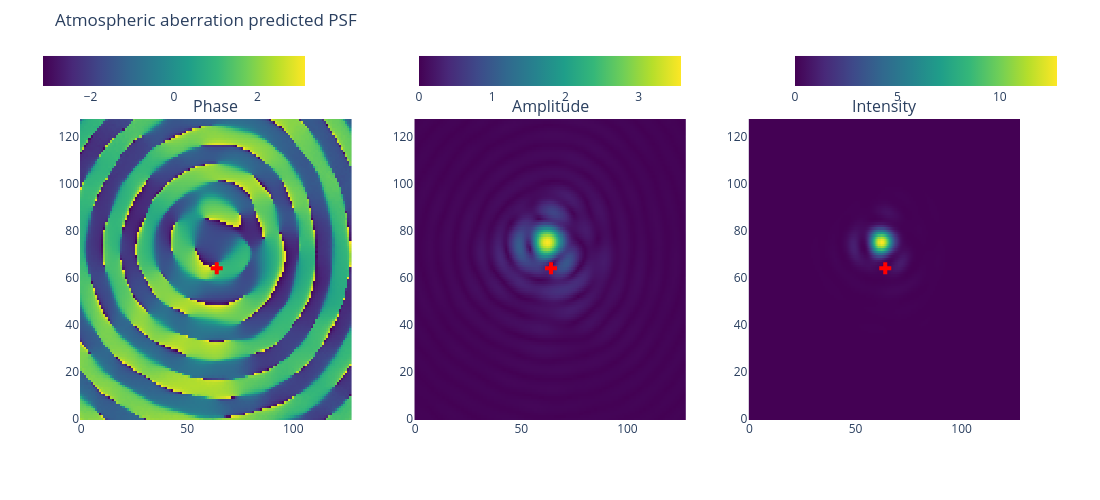
\includegraphics[width=0.4\textwidth]{pid-atmosphericaberrationpredictedpsf.png}
					\caption{Example original sized predicted PSF}\hspace{\fill}
				\end{figure*}			
				\item \textbf{Cropped sized predicted PSF}: A dataset of 70000 predicted electric fields stored in 64x64x2 matrices. These cropped predicted PSFs are the outputs of a model trained with the Cropped sized PSFs dataset and their corresponding PL intensities (which are the same ouput intensities from the Original sized PSFs dataset).
				\begin{figure*}[ht!]
					\centering
					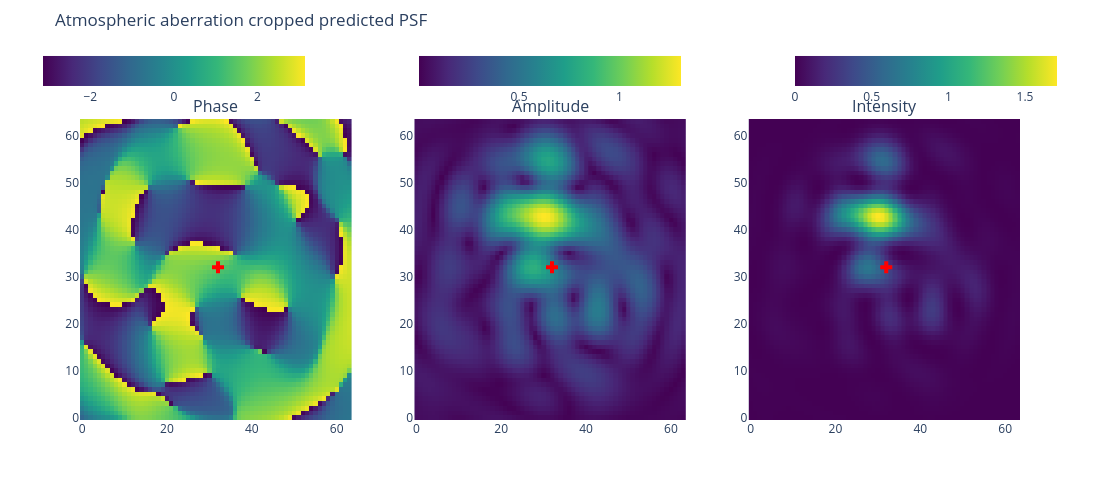
\includegraphics[width=0.4\textwidth]{pid-atmosphericaberrationcroppedpredictedpsf.png}
					\caption{Example cropped sized predicted PSF}\hspace{\fill}
				\end{figure*}
				\FloatBarrier			
			\end{itemize}
			
			
		\subparagraph{PL intensities}
		The same dataset of PL output intensities are used for every PSF dataset. The intensities are computed multiplying the LP coefficients by the transfer matrix of the \textbf{19 mode PL}. This dataset has 70000 datapoints, each datapoint being a vector of 19 elements.
		
	\subsubsection{Zernike modes related}
		There are 5 subgroups of datasets: PSFs generated with 2, 5, 9, 14 and 20 zernike modes. Each subgroup is divided in original sized, cropped sized, predicted and cropped predicted as in the case of the atmospheric aberration PSFs.
		\subparagraph{PSFs}
			\begin{itemize}
				\item \textbf{Original sized 2 modes PSFs}: A dataset of 70000 electric fields stored in 128x128x2 matrixes. The aberration by a 2 modes zernike basis.
				\begin{figure*}[ht!]
					\centering
					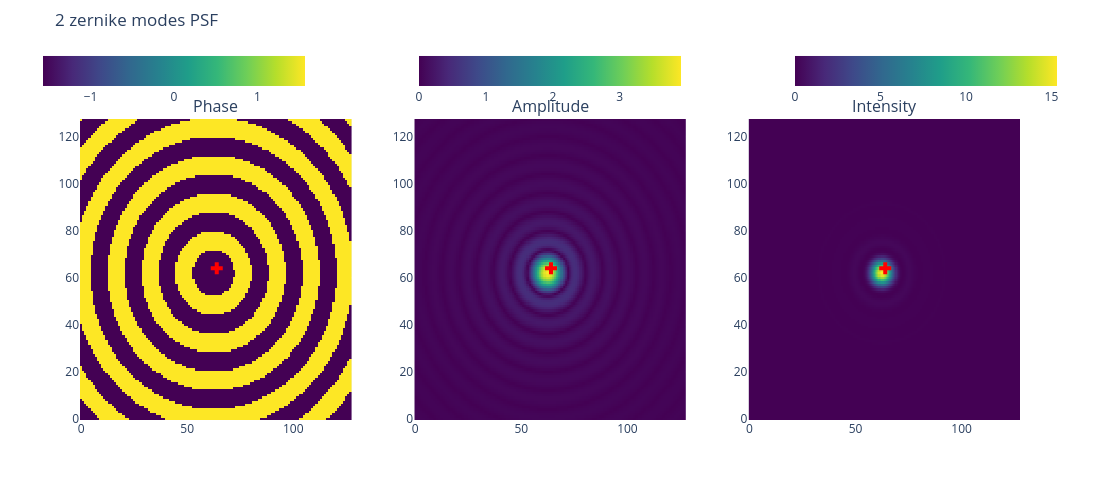
\includegraphics[width=0.4\textwidth]{pid-2mpsf.png}
					\caption{Example original sized 2 modes PSF}\hspace{\fill}
				\end{figure*}				
				\item \textbf{Cropped sized 2 modes PSFs}:  A dataset of 70000 electric fields stored in 64x64x2 matrixes. These cropped  PSFs correspond to the central pixels from the Original sized 2 modes PSFs.
				\begin{figure*}[ht!]
					\centering
					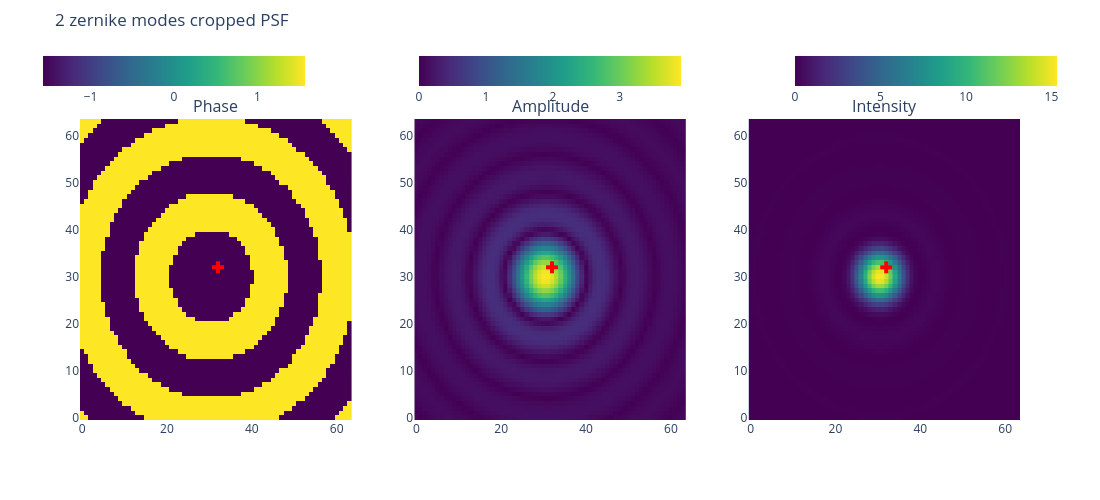
\includegraphics[width=0.4\textwidth]{pid-2mcroppedpsf.png}
					\caption{Example Cropped sized 2 modes PSF}\hspace{\fill}
				\end{figure*}			
				\item \textbf{Original sized predicted 2 modes PSFs}:  A dataset of 70000 predicted electric fields stored in 128x128x2 matrices. These predicted PSFs are the outputs of a model trained with the Original sized 2 modes PSFs dataset and their corresponding PL intensities.
				\begin{figure*}[ht!]
					\centering
					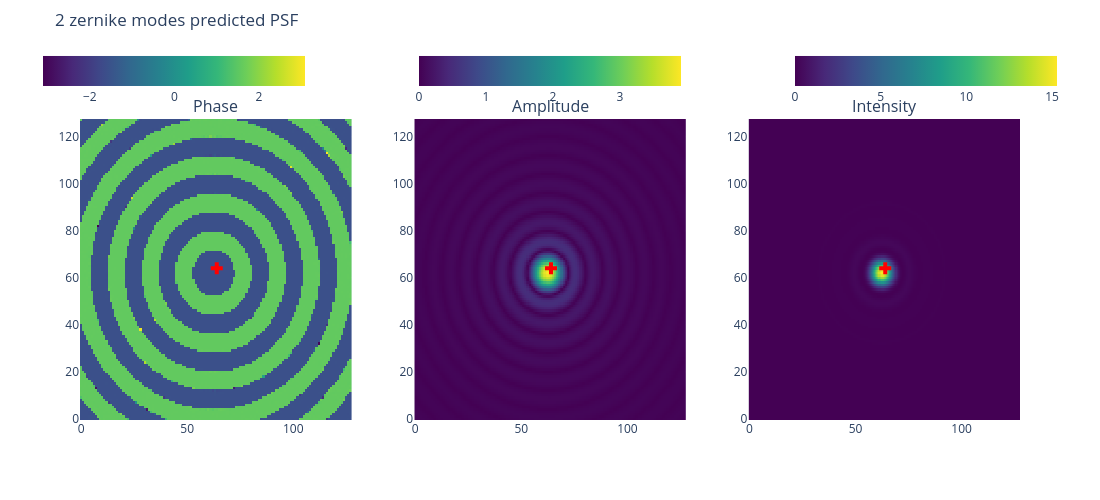
\includegraphics[width=0.4\textwidth]{pid-2mpredictedpsf.png}
					\caption{Example original sized predicted 2 modes PSF}\hspace{\fill}
				\end{figure*}			
				\item \textbf{Cropped sized predicted 2 modes PSF}: A dataset of 70000 predicted electric fields stored in 64x64x2 matrices. These cropped predicted PSFs are the outputs of a model trained with the Cropped sized 2 modes PSFs dataset and their corresponding PL intensities (which are the same ouput intensities from the Original sized 2 modes PSFs dataset).
				\begin{figure*}[ht!]
					\centering
					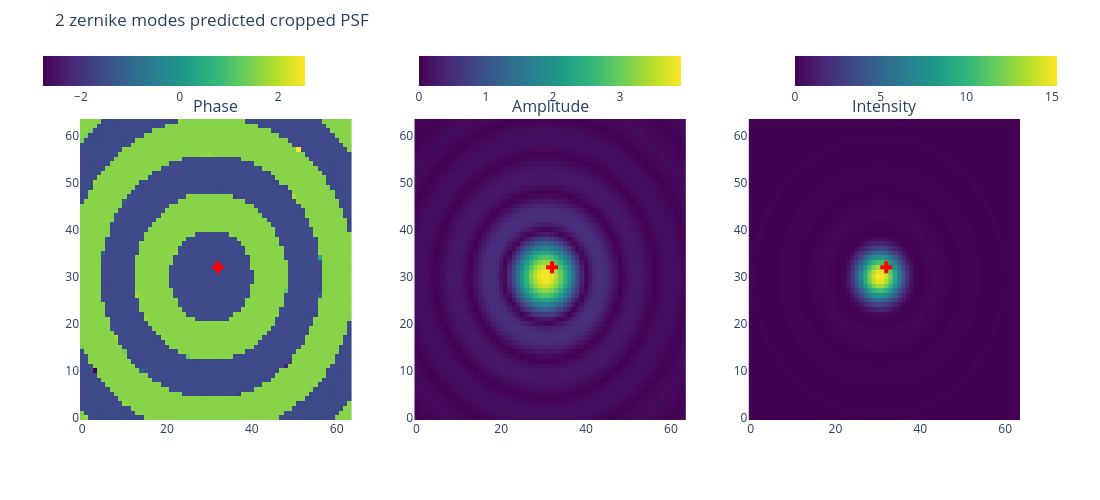
\includegraphics[width=0.4\textwidth]{pid-2mpredictedcroppedpsf.png}
					\caption{Example cropped sized predicted 2 modes PSF}\hspace{\fill}
				\end{figure*}
				\FloatBarrier
				
				\item \textbf{Original sized 5 modes PSFs}: A dataset of 70000 electric fields stored in 128x128x2 matrixes. The aberration by a 5 modes zernike basis.
				\begin{figure*}[ht!]
					\centering
					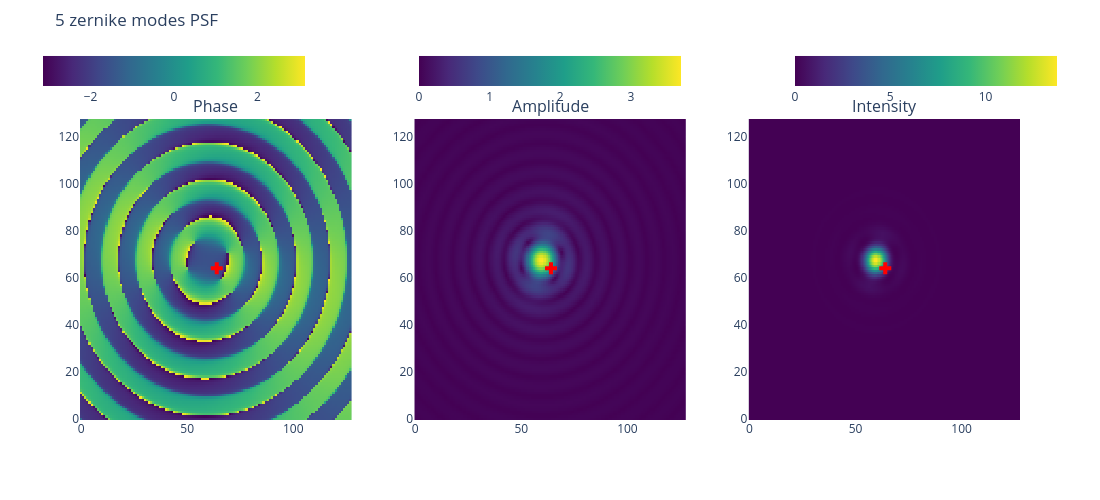
\includegraphics[width=0.4\textwidth]{pid-5mpsf.png}
					\caption{Example original sized 5 modes PSF}\hspace{\fill}
				\end{figure*}				
				\item \textbf{Cropped sized 5 modes PSFs}:  A dataset of 70000 electric fields stored in 64x64x2 matrixes. These cropped  PSFs correspond to the central pixels from the Original sized 5 modes PSFs.
				\begin{figure*}[ht!]
					\centering
					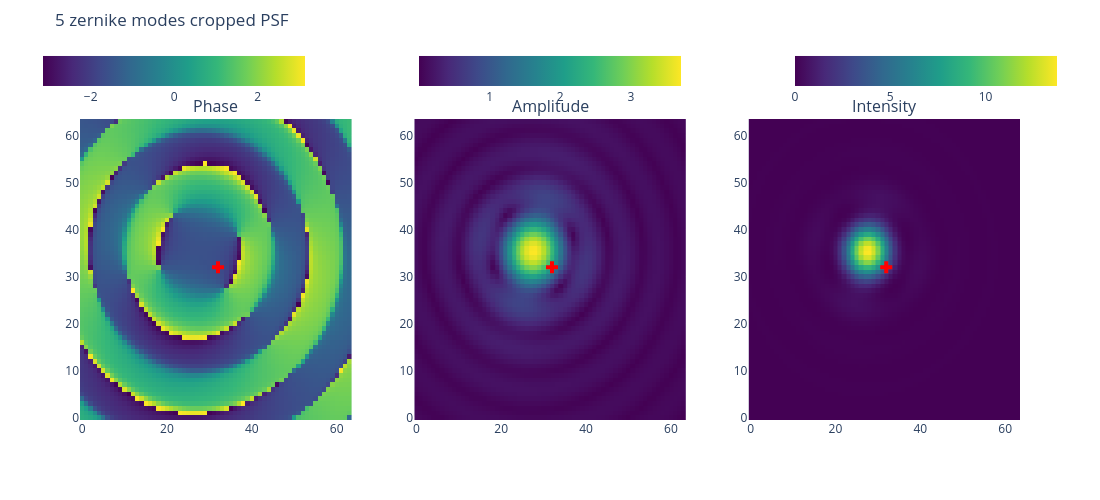
\includegraphics[width=0.4\textwidth]{pid-5mcroppedpsf.png}
					\caption{Example Cropped sized 5 modes PSF}\hspace{\fill}
				\end{figure*}			
				\item \textbf{Original sized predicted 5 modes PSFs}:  A dataset of 70000 predicted electric fields stored in 128x128x2 matrices. These predicted PSFs are the outputs of a model trained with the Original sized 5 modes PSFs dataset and their corresponding PL intensities.
				\begin{figure*}[ht!]
					\centering
					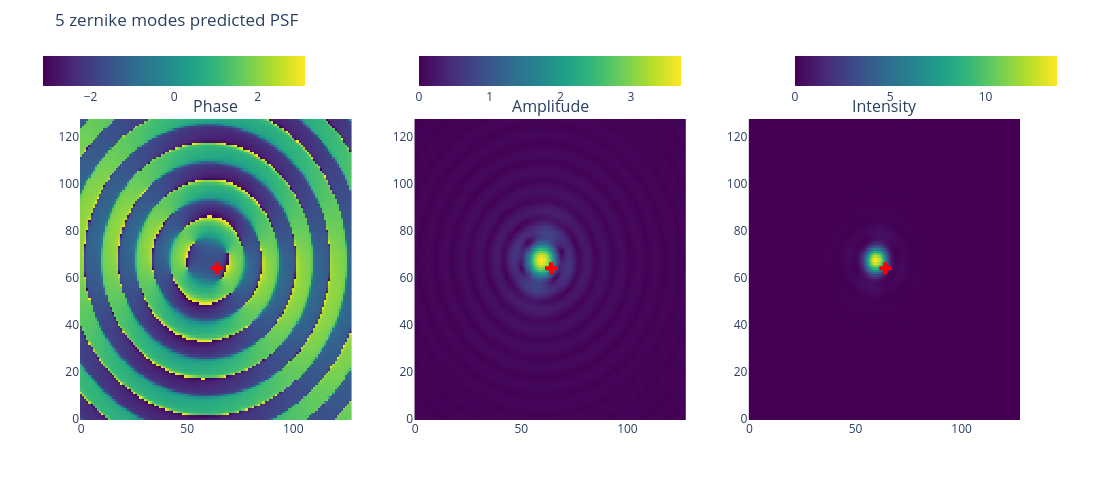
\includegraphics[width=0.4\textwidth]{pid-5mpredictedpsf.png}
					\caption{Example original sized predicted 5 modes PSF}\hspace{\fill}
				\end{figure*}			
				\item \textbf{Cropped sized predicted 5 modes PSF}: A dataset of 70000 predicted electric fields stored in 64x64x2 matrices. These cropped predicted PSFs are the outputs of a model trained with the Cropped sized 5 modes PSFs dataset and their corresponding PL intensities (which are the same ouput intensities from the Original sized 5 modes PSFs dataset).
				\begin{figure*}[ht!]
					\centering
					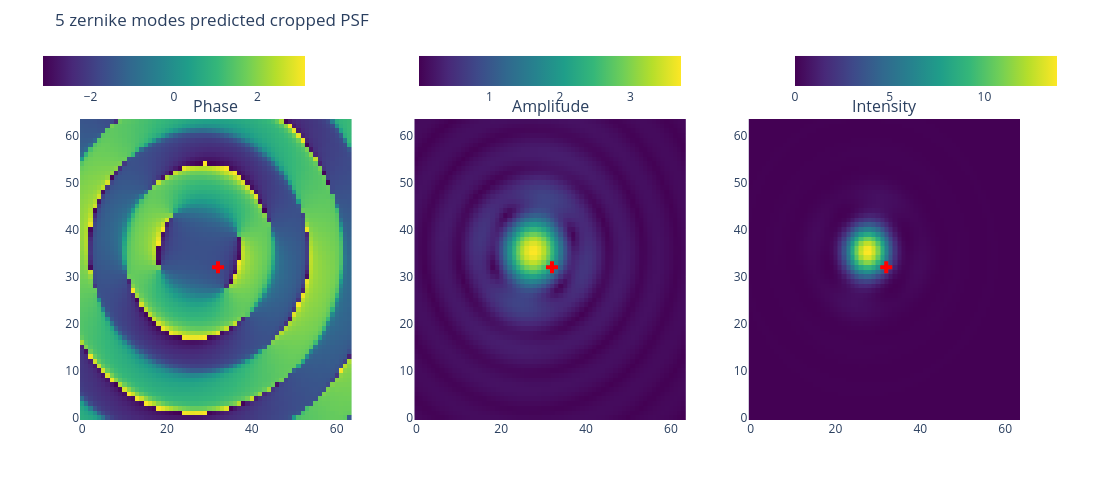
\includegraphics[width=0.4\textwidth]{pid-5mpredictedcroppedpsf.png}
					\caption{Example cropped sized predicted 5 modes PSF}\hspace{\fill}
				\end{figure*}
				\FloatBarrier
				
				\item \textbf{Original sized 9 modes PSFs}: A dataset of 70000 electric fields stored in 128x128x2 matrixes. The aberration by a 9 modes zernike basis.
				\begin{figure*}[ht!]
					\centering
					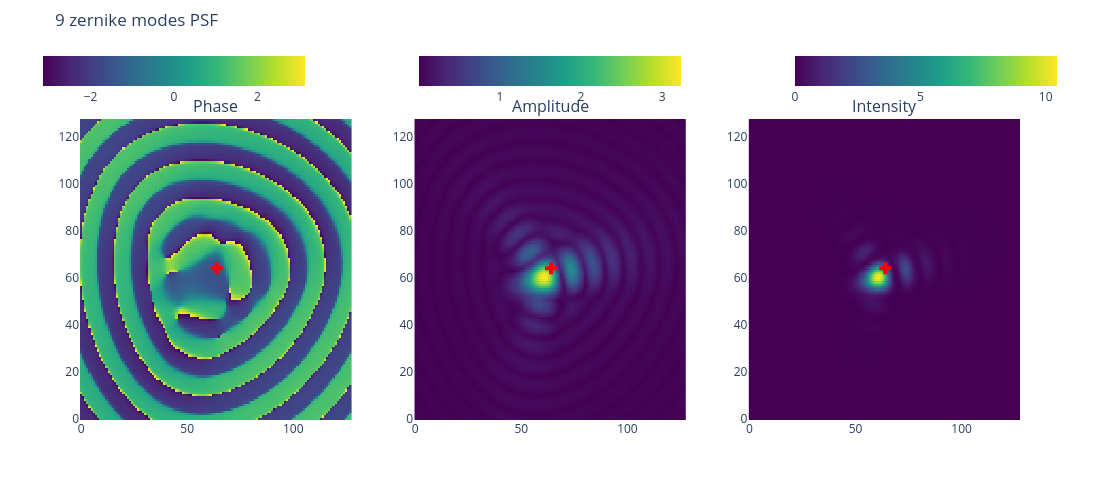
\includegraphics[width=0.4\textwidth]{pid-9mpsf.png}
					\caption{Example original sized 9 modes PSF}\hspace{\fill}
				\end{figure*}				
				\item \textbf{Cropped sized 9 modes PSFs}:  A dataset of 70000 electric fields stored in 64x64x2 matrixes. These cropped  PSFs correspond to the central pixels from the Original sized 9 modes PSFs.
				\begin{figure*}[ht!]
					\centering
					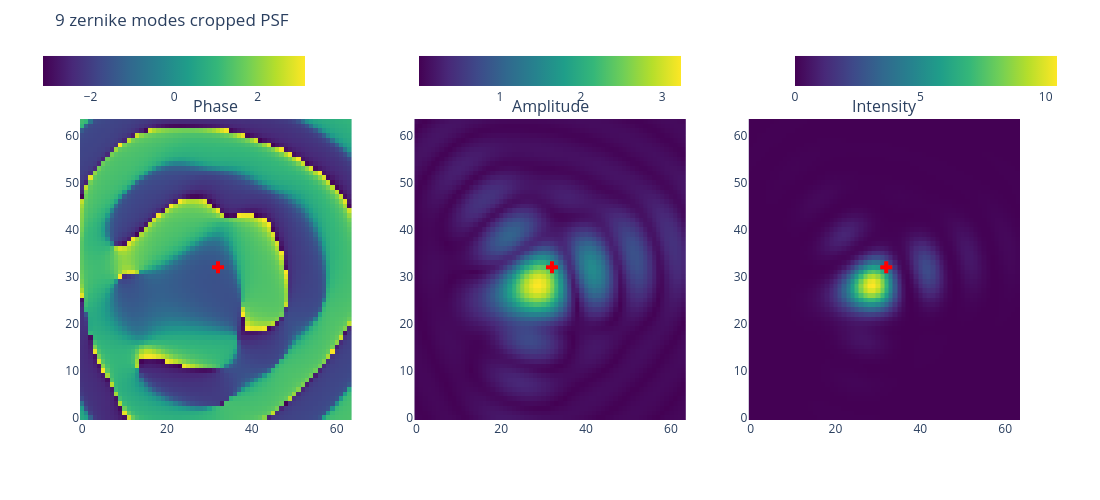
\includegraphics[width=0.4\textwidth]{pid-9mcroppedpsf.png}
					\caption{Example Cropped sized 9 modes PSF}\hspace{\fill}
				\end{figure*}			
				\item \textbf{Original sized predicted 9 modes PSFs}:  A dataset of 70000 predicted electric fields stored in 128x128x2 matrices. These predicted PSFs are the outputs of a model trained with the Original sized 9 modes PSFs dataset and their corresponding PL intensities.
				\begin{figure*}[ht!]
					\centering
					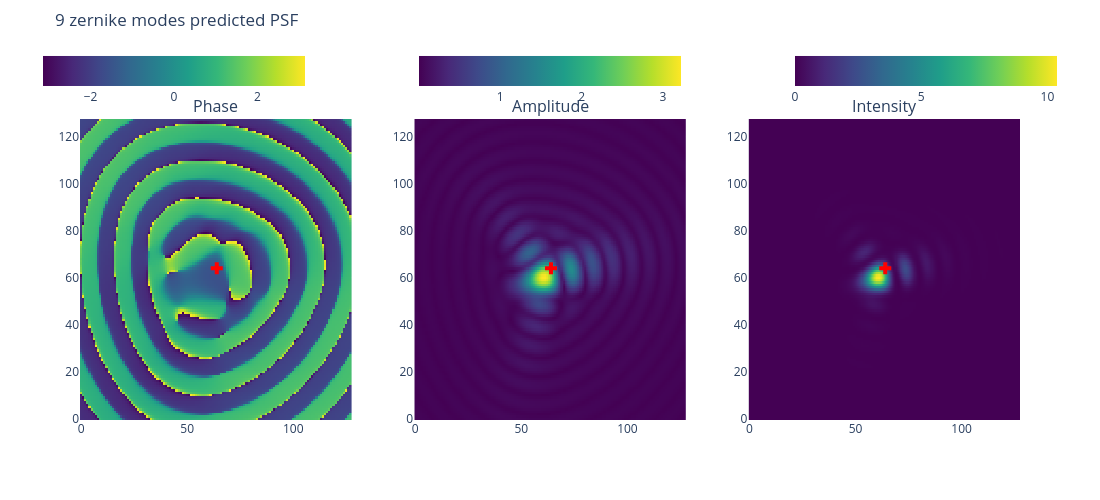
\includegraphics[width=0.4\textwidth]{pid-9mpredictedpsf.png}
					\caption{Example original sized predicted 9 modes PSF}\hspace{\fill}
				\end{figure*}			
				\item \textbf{Cropped sized predicted 9 modes PSF}: A dataset of 70000 predicted electric fields stored in 64x64x2 matrices. These cropped predicted PSFs are the outputs of a model trained with the Cropped sized 9 modes PSFs dataset and their corresponding PL intensities (which are the same ouput intensities from the Original sized 9 modes PSFs dataset).
				\begin{figure*}[ht!]
					\centering
					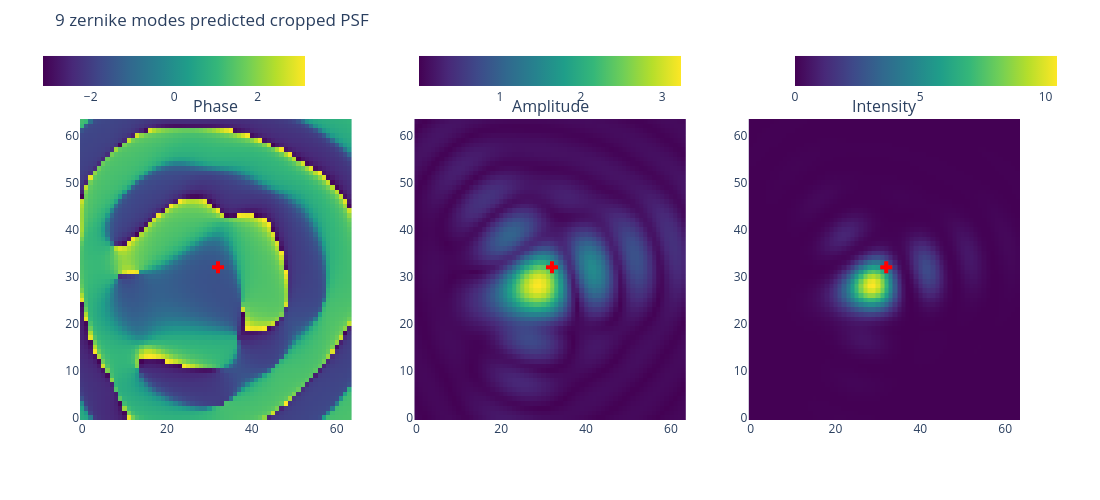
\includegraphics[width=0.4\textwidth]{pid-9mpredictedcroppedpsf.png}
					\caption{Example cropped sized predicted 9 modes PSF}\hspace{\fill}
				\end{figure*}
				\FloatBarrier
				
				\item \textbf{Original sized 14 modes PSFs}: A dataset of 70000 electric fields stored in 128x128x2 matrixes. The aberration by a 14 modes zernike basis.
				\begin{figure*}[ht!]
					\centering
					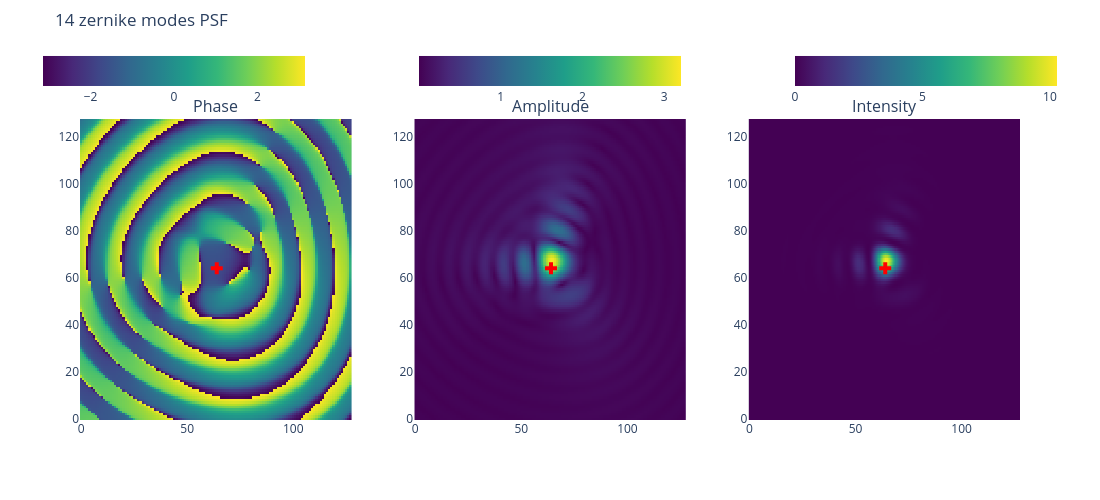
\includegraphics[width=0.4\textwidth]{pid-14mpsf.png}
					\caption{Example original sized 14 modes PSF}\hspace{\fill}
				\end{figure*}				
				\item \textbf{Cropped sized 14 modes PSFs}:  A dataset of 70000 electric fields stored in 64x64x2 matrixes. These cropped  PSFs correspond to the central pixels from the Original sized 14 modes PSFs.
				\begin{figure*}[ht!]
					\centering
					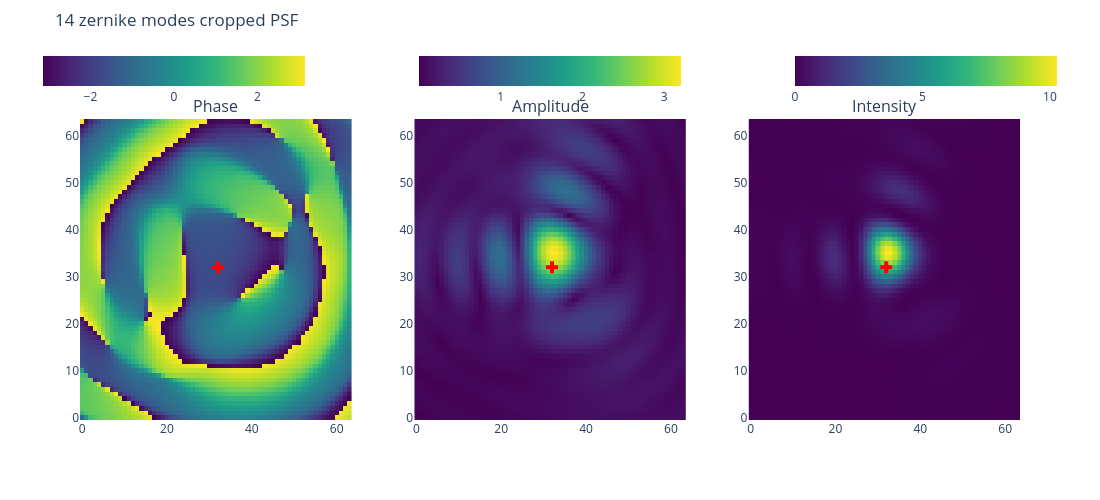
\includegraphics[width=0.4\textwidth]{pid-14mcroppedpsf.png}
					\caption{Example Cropped sized 14 modes PSF}\hspace{\fill}
				\end{figure*}			
				\item \textbf{Original sized predicted 14 modes PSFs}:  A dataset of 70000 predicted electric fields stored in 128x128x2 matrices. These predicted PSFs are the outputs of a model trained with the Original sized 14 modes PSFs dataset and their corresponding PL intensities.
				\begin{figure*}[ht!]
					\centering
					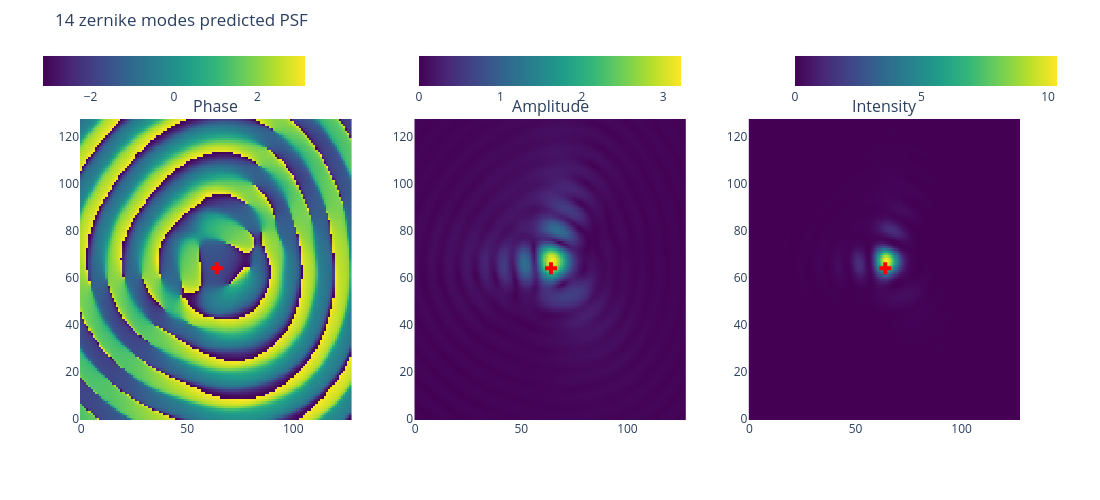
\includegraphics[width=0.4\textwidth]{pid-14mpredictedpsf.png}
					\caption{Example original sized predicted 14 modes PSF}\hspace{\fill}
				\end{figure*}			
				\item \textbf{Cropped sized predicted 14 modes PSF}: A dataset of 70000 predicted electric fields stored in 64x64x2 matrices. These cropped predicted PSFs are the outputs of a model trained with the Cropped sized 14 modes PSFs dataset and their corresponding PL intensities (which are the same ouput intensities from the Original sized 14 modes PSFs dataset).
				\begin{figure*}[ht!]
					\centering
					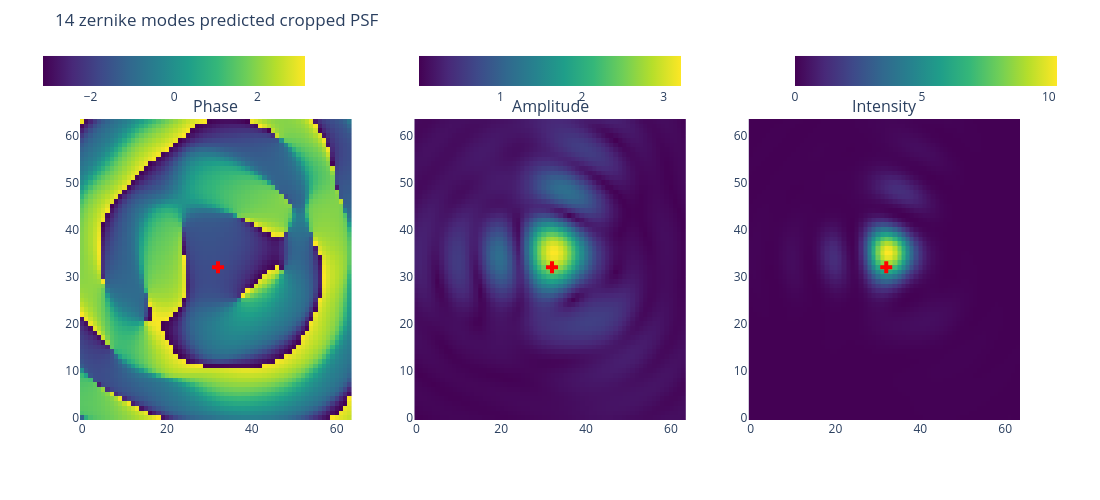
\includegraphics[width=0.4\textwidth]{pid-14mpredictedcroppedpsf.png}
					\caption{Example cropped sized predicted 14 modes PSF}\hspace{\fill}
				\end{figure*}
				\FloatBarrier
				
				\item \textbf{Original sized 20 modes PSFs}: A dataset of 70000 electric fields stored in 128x128x2 matrixes. The aberration by a 20 modes zernike basis.
				\begin{figure*}[ht!]
					\centering
					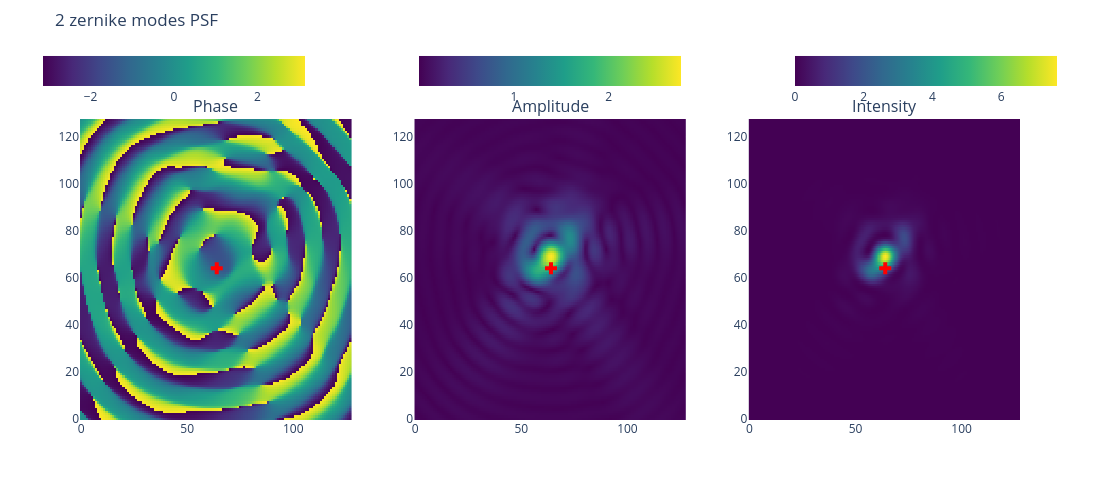
\includegraphics[width=0.4\textwidth]{pid-20mpsf.png}
					\caption{Example original sized 20 modes PSF}\hspace{\fill}
				\end{figure*}				
				\item \textbf{Cropped sized 20 modes PSFs}:  A dataset of 70000 electric fields stored in 64x64x2 matrixes. These cropped  PSFs correspond to the central pixels from the Original sized 20 modes PSFs.
				\begin{figure*}[ht!]
					\centering
					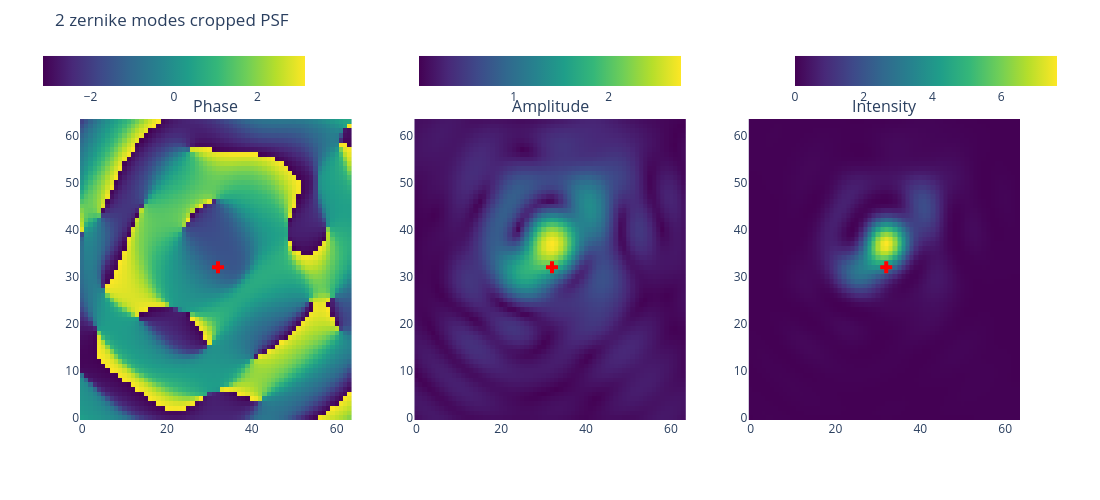
\includegraphics[width=0.4\textwidth]{pid-20mcroppedpsf.png}
					\caption{Example Cropped sized 20 modes PSF}\hspace{\fill}
				\end{figure*}			
				\item \textbf{Original sized predicted 20 modes PSFs}:  A dataset of 70000 predicted electric fields stored in 128x128x2 matrices. These predicted PSFs are the outputs of a model trained with the Original sized 20 modes PSFs dataset and their corresponding PL intensities.
				\begin{figure*}[ht!]
					\centering
					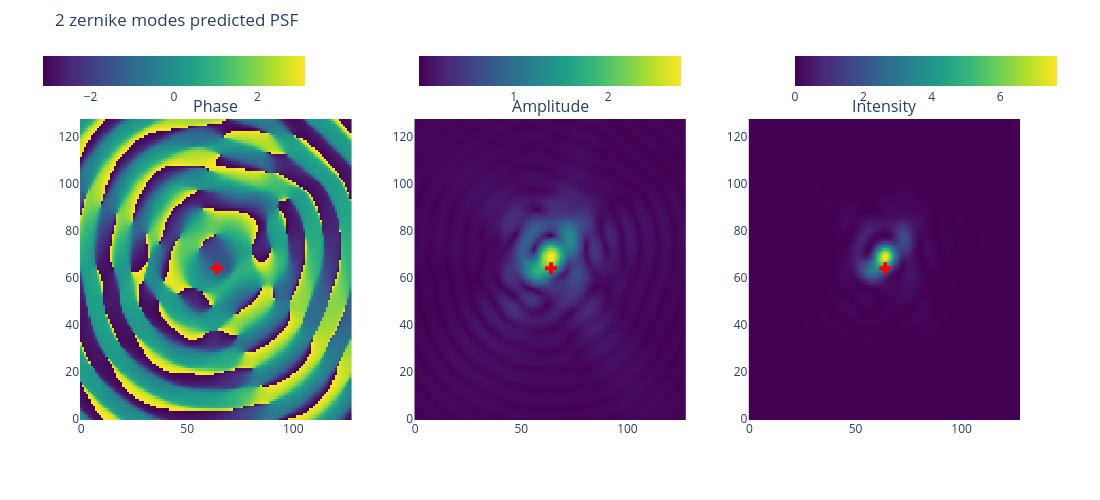
\includegraphics[width=0.4\textwidth]{pid-20mpredictedpsf.png}
					\caption{Example original sized predicted 20 modes PSF}\hspace{\fill}
				\end{figure*}			
				\item \textbf{Cropped sized predicted 20 modes PSF}: A dataset of 70000 predicted electric fields stored in 64x64x2 matrices. These cropped predicted PSFs are the outputs of a model trained with the Cropped sized 20 modes PSFs dataset and their corresponding PL intensities (which are the same ouput intensities from the Original sized 20 modes PSFs dataset).
				\begin{figure*}[ht!]
					\centering
					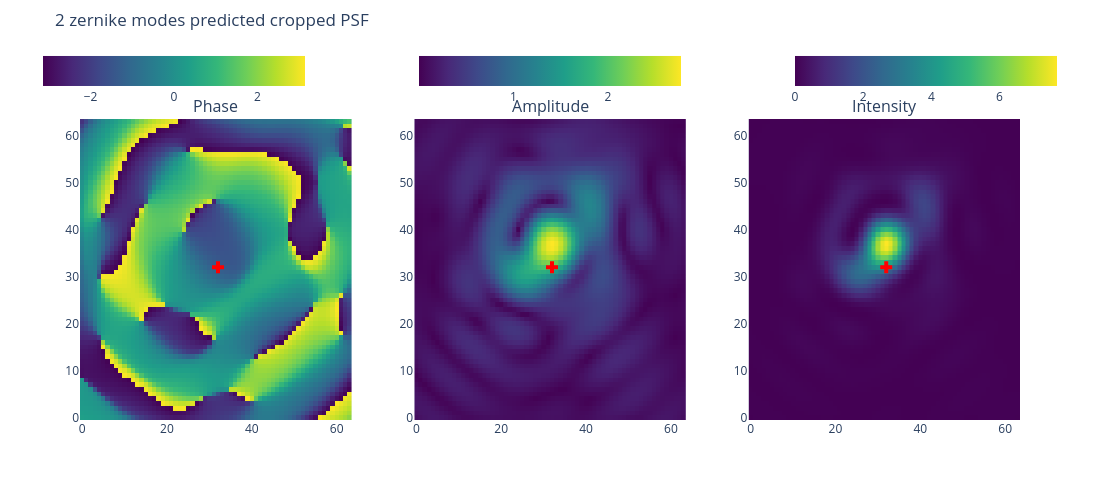
\includegraphics[width=0.4\textwidth]{pid-20mpredictedcroppedpsf.png}
					\caption{Example cropped sized predicted 20 modes PSF}\hspace{\fill}
				\end{figure*}
				\FloatBarrier
			\end{itemize}
			
		\subparagraph{LP mode coefficients}
			There are two PL intensities dataset per Zernike aberration PSF subgroup: LP modes coefficients for 2, 5, 9, 14, 20 modes PSFs. Each of the dataset has 70000 datapoints each datapoint being the complex coefficients stored in a 19x2 matrix that separates the real and imaginary part of the coefficients.\\
			
			The two datasets correspond to the LP coefficients that are computed in the multimode end of Photonic Lanterns. The PLs are:
			\begin{itemize}
				\item 19 mode supporting multimode end with 19 waveguides in the single mode end.
				\item 42 mode supporting multimode end with 42 waveguides in the single mode end.
			\end{itemize}
			
		\subparagraph{PL intensities}
		
			There is one PL intensities dataset per Zernike aberration PSF subgroup: PL intensities for 2, 5, 9, 14, 20 modes PSFs. Each of the dataset has 70000 datapoints each datapoint being the 19 intensities corresponding to the PSF
			
			The two datasets correspond to the single mode end intensities of Photonic Lanterns. The PLs are:
			\begin{itemize}
				\item 19 mode supporting multimode end with 19 waveguides in the single mode end.
				\item 42 mode supporting multimode end with 42 waveguides in the single mode end.
			\end{itemize}

\finishday